\documentclass[11pt]{article}
\usepackage[a4paper,total={6in,8in},margin=1in]{geometry}
\geometry{letterpaper}
\usepackage[utf8]{inputenc} % allow utf-8 input
\usepackage[T1]{fontenc}    % use 8-bit T1 fonts
\usepackage{microtype,inconsolata}
\usepackage{times,latexsym}
\usepackage{graphicx}
\usepackage{subfig}
\usepackage{amsmath,amssymb,mathabx,mathtools,amsthm,nicefrac}
\usepackage[linesnumbered,ruled,vlined]{algorithm2e}
\usepackage{enumitem}
\usepackage[pagebackref,breaklinks,colorlinks]{hyperref}
\usepackage[skip=3pt,font=small]{subcaption}
\usepackage[skip=3pt,font=small]{caption}
\usepackage[dvipsnames,svgnames,x11names,table]{xcolor}
\usepackage[capitalise,noabbrev,nameinlink]{cleveref}
\usepackage{booktabs,tabularx,colortbl,multirow,multicol,array,makecell,tabularray}
\usepackage[english]{babel}
\usepackage{listings}

\definecolor{color-C00000}{rgb}{0.75,0,0}
\definecolor{red}{rgb}{1,0,0}

\def\E{{\rm E}}
\def\Var{{\rm Var}}
\def\I{{\bf I}}
\def\w{{\bf w}}
\def\B{{\bf B}}
\def\b{{\bf b}}
\def\a{\alpha}
\def\tI{\tilde{\bf I}}
\def\tM{\tilde{M}}

\def\bF{{\bar{F}}}
\def\F{{\bf F}}

\def\D{{\cal D}}
\def\C{{\cal C}}
\def\S{{\cal S}}
\def\L{{\cal L}}

\def\obs{{\rm obs}}
\def\syn{{\rm syn}}

\begin{document}

\begin{center}
{\bf\Large Computer Vision I: Project 4 (10 points)}

\vspace{1em}
Due on Dec. 13th, 11:59pm

\vspace{1em}
2100017727 Keran Wang
\end{center}



\section{Background} 

This project is based on Section 11.1: Deep FRAME. Read the textbook for more information.

\subsection{Python Library}

Please install the latest matplotlib, pillow, scikit-image, torch and torchvision. You are also welcome to utilize any libraries of your choice, \textbf{but please report them in your report (for autograder)!}
\color{black}

\subsection{What to hand in?}

Please submit both a formal report and the accompanying code. For the report, kindly provide a PDF version. You may opt to compose a new report or complete the designated sections within this document, as can be started by simply loading the tex file to Overleaf. Your score will be based on the quality of \textbf{your results}, \textbf{the analysis} (diagnostics of issues and comparisons) of these results in your report, and your \textbf{code implementation}. You may delete all the images before handing them in, as they may be too large for the autograder.

\paragraph{Notice.} Do not modify the function names, parameters, and returns in the given code, unless explicitly specified in this document.

\subsection{Help}

Make a diligent effort to independently address any encountered issues, and in cases where challenges exceed your capabilities, do not hesitate to seek assistance! Collaboration with your peers is permitted, but it is crucial that you refrain from directly \textcolor{red}{examining or copying one another's code.}  Please be aware that you'll fail the course if our \textbf{code similarity checker}, which has found some prohibited behaviors before, detects these violations. For details, please refer to: \url{https://yzhu.io/s/teaching/plagiarism}.

\clearpage

\section{Introduction to Hierarchical FRAME Model}

 Notations. Let $\I(x)$ be an image defined on the square (or rectangular) image domain $\Lambda$, where $x = (x_1, x_2)$ indexes the coordinates of pixels. We can treat $\I(x)$ as a two-dimensional function defined on $\Lambda$. We can also treat $\I$ as a vector if we fix an ordering for the pixels. 

For a filter (or neuron) $F$, let $F*\I$ denote the filtered image or feature map, and let $[F*\I](x)$ denote the {\em filter response} or {\em feature} at position $x$. 

A hierarchical FRAME model is a composition of multiple layers of linear filtering and element-wise non-linear transformation  as expressed by the following recursive formula: 
\begin{equation}
	%\begin{aligned}
	[F^{(l)}_{k}  *\I](x)  =   h\left(\sum_{i=1}^{N_{l-1}}  \sum_{y \in \S_{l}} w^{(l, k)}_{i, y}   [F^{(l-1)}_{i}*\I](x+y) + b_{l, k}\right) \\
	%\end{aligned}
	\label{eq:ConvNet}
\end{equation}
where $l \in \{1, 2, ..., {\cal L}\}$ indexes the layer.  $\{F^{(l)}_k, k = 1, ..., N_l\}$ are the filters at layer $l$, and $\{F^{(l-1)}_i, i = 1, ..., N_{l-1}\}$ are the filters at layer $l-1$. $b_{l,k}$ is the bias term. $k$ and $i$ are used to index filters at layers $l$ and $l-1$ respectively, and $N_l$ and $N_{l-1}$ are the numbers of filters at layers $l$ and $l-1$ respectively. The filters are locally supported, so the range of $y$  is within a local support $\S_{l}$  (such as a $7 \times 7$ image patch). At the bottom layer, $[F^{(0)}_k*\I](x) = \I_k(x)$, where $k \in \{R, G, B\}$ indexes the three color channels. Sub-sampling may be implemented so that in  $[F^{(l)}_{k}  *\I](x)$, $x \in \Lambda_l \subset \Lambda$. 

We take $h(r) = \max(r, 0)$, the rectified linear unit (re-lu), as is commonly adopted in ConvNet. We define the following random field model as the hierarchical FRAME model:
\begin{equation}
p(\I; w) = \frac{1}{Z(w)} \exp \left[\sum_{k=1}^{K} \sum_{x \in \Lambda_L} [F_k^{(L)}*\I](x)\right] q(\I), 
\label{eq:ConvNet-FRAME}
\end{equation}
where  $w = (\w_k, b_k, k = 1, ..., K)$ are the filters at the top layer.  $q(\I)$ is the Gaussian white noise model.

% includes parameters in all layers with $\w_k=\{ w^{(l, k)}_{i, y} \}$ denoting all the filters at layer $k$ and $b_k=\{ b_{l,k}\}$ all the bias (threshold) at filters in layer $k$.  $h(r) = \max(r, 0)$. 

 
Model (\ref{eq:ConvNet-FRAME})  corresponds to the exponential tilting model with scoring function
\begin{equation}
f(\I; w) = \sum_{k=1}^{K} \sum_{x \in \Lambda_L} [F_k^{(L)}*\I](x). \label{eq:a}
\end{equation}

The learning of $w$ from training images $\{\I_m, m = 1, ..., M\}$  can be accomplished by maximum likelihood. In our case, we have only 1 image for training, i.e. $M=1$.
 Let $L(w) = \sum_{m=1}^{M} \log p(\I; w)/M$, 
\begin{equation}
	%\begin{aligned}
	\frac{\partial L(w)}{\partial w} = \frac{1}{M} \sum_{m=1}^{M} \frac{\partial}{\partial w} f(\I_m; w) 
	-  \E_{p(I)} \left[ \frac{\partial}{\partial w} f(\I; w) \right].
	%\end{aligned}
\label{eq:grad}
\end{equation}


The expectation can be approximated by Monte Carlo samples. One can sample from $p(\I; w)$ in (\ref{eq:ConvNet-FRAME}) by the Langevin dynamics: 
\begin{equation}
\I_{\tau+1} = \I_{\tau} - \frac{\epsilon^2}{2} \left[\I_\tau - \frac{\partial}{\partial \I}f(\I; w) \right] + \epsilon Z_\tau,
\end{equation}
where $\tau$ denotes the time step, $\epsilon$ denotes the step size, assumed to be sufficiently small, $Z_\tau \sim {\rm N}(0, {\bf 1})$.

We can build up the model layer by layer. 
Given the filters at layers below, the top layer weight and bias parameters can be learned according to 
\begin{equation}
\begin{aligned}
\frac{\partial L(w)}{\partial w_{i, y}^{(L, k)}} =& \frac{1}{M} \sum_{m=1}^{M}\sum_{x \in \Lambda_L} \delta^{(L)}_{k, x}(\I_m; w)  [F^{(L-1)}_{i} * \I_m](x+y) \\
&   -  \frac{1}{\tilde{M}} \sum_{m=1}^{\tilde{M}} \sum_{x \in \Lambda_L} \delta^{(L)}_{k, x}(\tilde{\I}_m; w)  [F^{(L-1)}_{i} * \tilde{\I}_m](x+y), \\
\end{aligned}
\label{eq:generativeGradient}
\end{equation}
and
\begin{equation}
\begin{aligned}
\frac{\partial L(w)}{\partial b_{L, k}} = \frac{1}{M} \sum_{m=1}^{M}\sum_{x \in \Lambda_L} \delta^{(L)}_{k, x}(\I_m; w) - \frac{1}{\tilde{M}} \sum_{m=1}^{\tilde{M}} \sum_{x  \in \Lambda_L} \delta^{(L)}_{k, x}(\tilde{\I}_m; w).
\end{aligned}
\label{eq:generativeGradient0}
\end{equation}
where $\I_m$ are $M$ observed images, and $\tilde{\I}_m$ are $\tilde{M}$ synthesized images sampled from the model. Here, we choose $M=\tilde{M}=1$. Hint: you can leverage an automatic differentiation engine to simplify the computation of gradients, \textit{e.g.}, PyTorch.

\section{Experiment}
For one of the input images, you will learn a hierarchical FRAME model. We define the Julesz ensemble as the set of images that reproduce the observed sufficient statistics over those designed filters. You use Langevin dynamics (code is given) to draw samples from the model. Figure~\ref{fig:syn} shows an example of synthesis. The synthesis starts from a zero image and the sampling stops when it matches all the sufficient statistics. To reduce the computational complexity, all images are resized into the size of $224\times 224$ pixels.

\begin{figure}[h]
	\centering
	\setlength{\fboxrule}{1pt}
	\setlength{\fboxsep}{0cm}	
	\subfloat{
		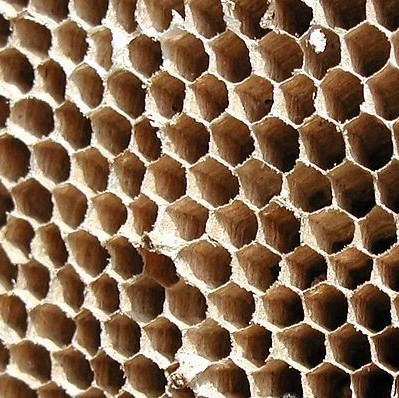
\includegraphics[width=.16\linewidth]{images/beehive.jpg}
		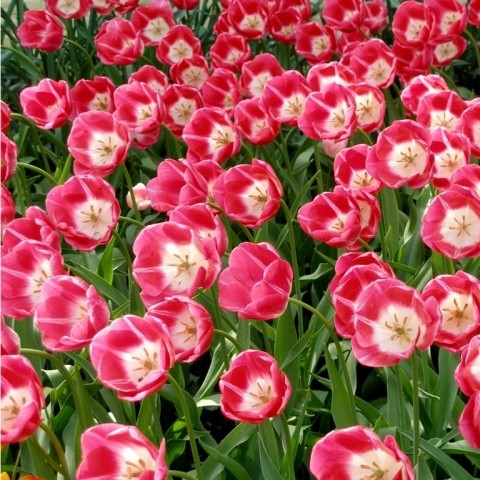
\includegraphics[width=.16\linewidth]{images/rose.jpg}
		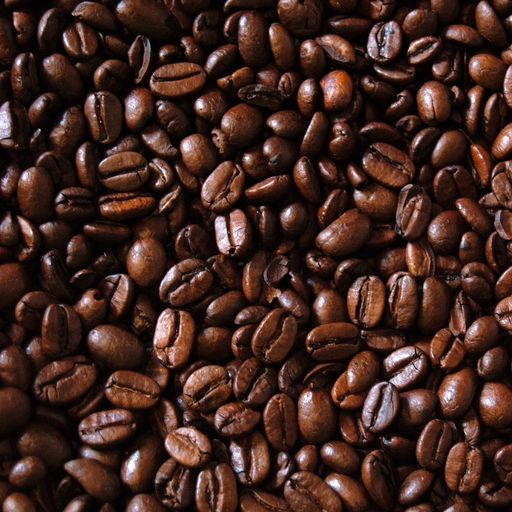
\includegraphics[width=.16\linewidth]{images/coffee.jpg}
		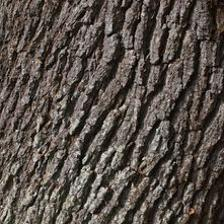
\includegraphics[width=.16\linewidth]{images/bark.jpg}
		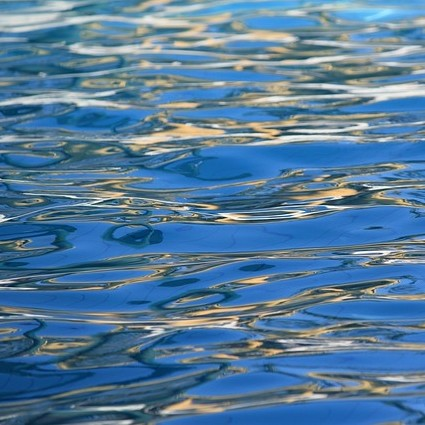
\includegraphics[width=.16\linewidth]{images/water.jpg}
		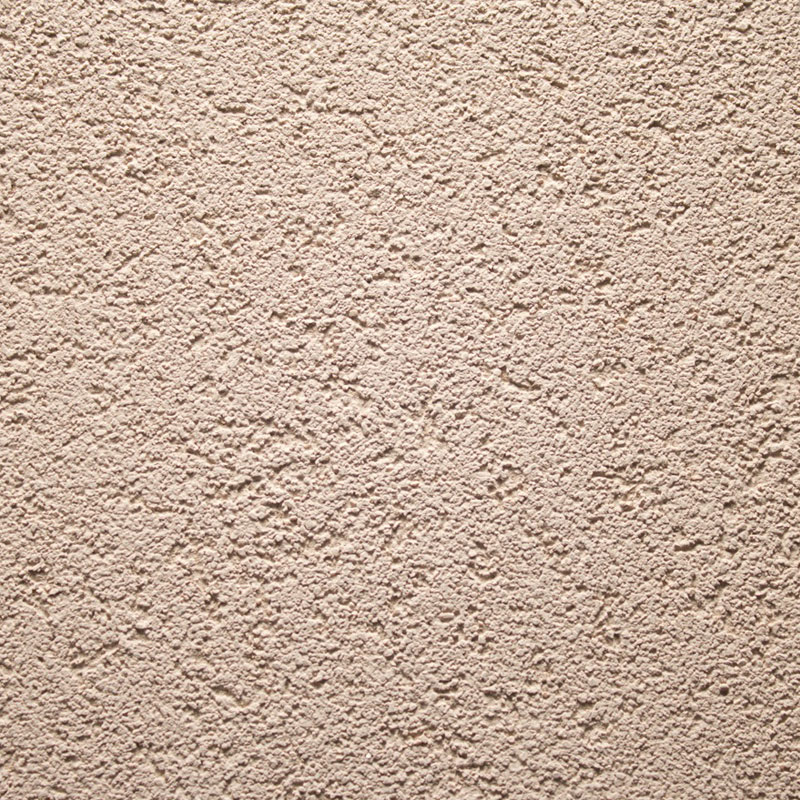
\includegraphics[width=.16\linewidth]{images/stucco.jpg}
	}\\[3px]
	\caption{Six images: from low entropy(sparse regime) to high entropy (Gibbs regime).}
\end{figure}

\begin{figure}[h]
	\centering
	\setlength{\fboxrule}{1pt}
	\setlength{\fboxsep}{0cm}	
	\subfloat{
		\includegraphics[width=.22\linewidth]{images/rose_small.jpg}
		\includegraphics[width=.22\linewidth]{images/layer_1.png}
		\includegraphics[width=.22\linewidth]{images/layer_2.png}
		\includegraphics[width=.22\linewidth]{images/layer_3.png}
	}\\[3px]
	\caption{Synthesis example. The first image is the training image, and from left to right, the rest images are synthesized images using 1, 2, and 3 layers respectively.}
	\label{fig:syn}
\end{figure}

\section{Code}
An overview of the learning of deep FRAME model:
\begin{enumerate}
    \item Given a target image that specifies a type of texture, our goal is to model the statistics of this texture and thereby synthesize a similar image.
    \item The distribution of the image is governed by a FRAME model, with the exponential term determined by a neural descriptor (CNN). The objective is to maximize the likelihood of target image under this distribution. And the gradient w.r.t. the descriptor is derived as in \cref{eq:grad}, where the first term can be computed by leveraging autograd and the second term can be approximated via Langevin dynamics.
    \item Starting from a zero-initialized image, we keep iterating the synthetic image. During each round of training, we first update the synthetic image with a better one via Langevin dynamics. Then with this updated synthetic image, we compute $f(I_{tgt})-f(I_{syn})$, backward the loss, and update the parameters of descriptor.
    \item Notably, the objective to be maximized $f(I_{tgt})-f(I_{syn})$ would probably oscillate instead of increasing monotonously. This is because sampling the synthetic image via Langevin dynamics would lead to larger $f(I_{syn})$, despite the gradient ascent when updating descriptor parameters.
\end{enumerate}

The training images locate at \texttt{images/}. The experimental results will be saved at a folder named according to the configurations, \textit{e.g.}, \texttt{rose\_3layer} (modeling rose texture with a 3-layer encoder). \texttt{deep\_frame.py} is the main entry function, which gives an example of learning and synthesizing images from the model. Running this python file requires two arguments, one specifying the number of layers and the other specifying the image tag. For example, train a 3-layer deep FRAME model on rose:
\begin{lstlisting}
python deep_frame.py --layer 3 --tag rose
\end{lstlisting}

\textbf{Modification:} You design your own structures of the model with 1 and 2 convolutional layers. The example setting may not generate vivid results. You might need to adjust the learning rates and sampling step size of the Langevin dynamics.

The code will determine GPU capabilities and fall back to CPU computation automatically.


\section{Submission: results and analysis}

In your submission, please provide the following:
\begin{enumerate}
    \item Show the synthesized images with 1,2,3 layers on the beehive image for your best design.
    \item Display the filters in the first layer using your visualization function. Compare these filters across the images. For some selected images, try to compare the learned filtered in different designs.
    \item Submit your completed code.
\end{enumerate}

\subsection{Synthesized Images}
\begin{figure}[h]
	\centering
	\setlength{\fboxrule}{1pt}
	\setlength{\fboxsep}{0cm}	
	\subfloat{
		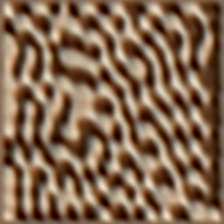
\includegraphics[width=.18\linewidth]{images/beehive_1layer/400.png}
		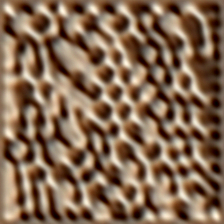
\includegraphics[width=.18\linewidth]{images/beehive_1layer/800.png}
		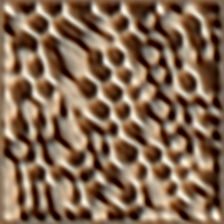
\includegraphics[width=.18\linewidth]{images/beehive_1layer/1200.png}
		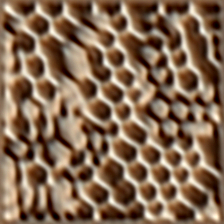
\includegraphics[width=.18\linewidth]{images/beehive_1layer/1600.png}
        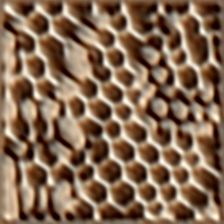
\includegraphics[width=.18\linewidth]{images/beehive_1layer/2000.png}
	}\\[3px]
	\caption{Synthesized Images for 1 layer: from epoch 400 to epoch 2000}
\end{figure}
\begin{figure}[h]
	\centering
	\setlength{\fboxrule}{1pt}
	\setlength{\fboxsep}{0cm}	
	\subfloat{
		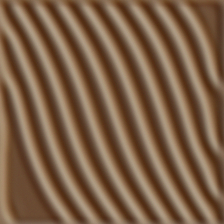
\includegraphics[width=.18\linewidth]{images/beehive_2layer/400.png}
		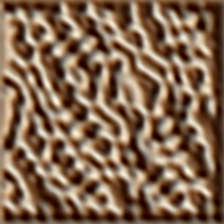
\includegraphics[width=.18\linewidth]{images/beehive_2layer/800.png}
		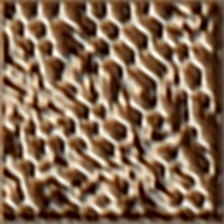
\includegraphics[width=.18\linewidth]{images/beehive_2layer/1200.png}
		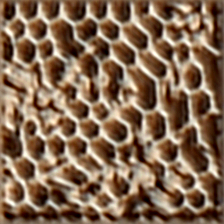
\includegraphics[width=.18\linewidth]{images/beehive_2layer/1600.png}
        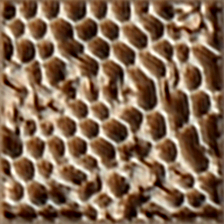
\includegraphics[width=.18\linewidth]{images/beehive_2layer/2000.png}
	}\\[3px]
	\caption{Synthesized Images for 2 layers: from epoch 400 to epoch 2000}
\end{figure}
\begin{figure}[h]
	\centering
	\setlength{\fboxrule}{1pt}
	\setlength{\fboxsep}{0cm}	
	\subfloat{
		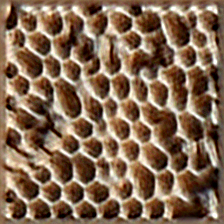
\includegraphics[width=.18\linewidth]{images/beehive_3layer/400.png}
		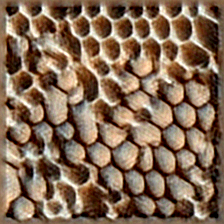
\includegraphics[width=.18\linewidth]{images/beehive_3layer/800.png}
		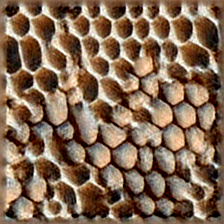
\includegraphics[width=.18\linewidth]{images/beehive_3layer/1200.png}
		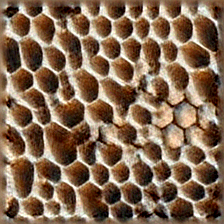
\includegraphics[width=.18\linewidth]{images/beehive_3layer/1600.png}
        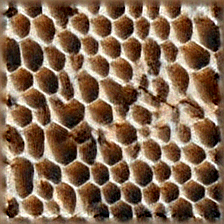
\includegraphics[width=.18\linewidth]{images/beehive_3layer/2000.png}
	}\\[3px]
	\caption{Synthesized Images for 3 layers: from epoch 400 to epoch 2000}
\end{figure}
From the images, we can see that Deep FRAME with 3 layers is enough for synthesizing the picture.
\subsection{Filters}
Three conv images are shown below:
\begin{figure}[h]
	\centering
	\setlength{\fboxrule}{1pt}
	\setlength{\fboxsep}{0cm}	
	\subfloat{
		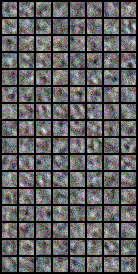
\includegraphics[width=.3\linewidth]{images/beehive_1layer/conv1.png}
		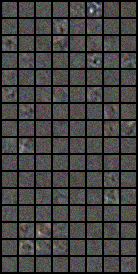
\includegraphics[width=.3\linewidth]{images/beehive_2layer/conv1.png}
		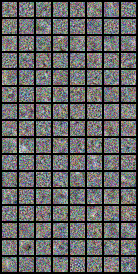
\includegraphics[width=.3\linewidth]{images/beehive_3layer/conv1.png}
	}\\[3px]
	\caption{Filters for beehive: from 1 layer to 3 layers}
\end{figure}
We can discover that, with more layers, the filtered image will be more clear.
We can also compare different filters between images:
\begin{figure}[h]
	\centering
	\setlength{\fboxrule}{1pt}
	\setlength{\fboxsep}{0cm}	
	\subfloat{
		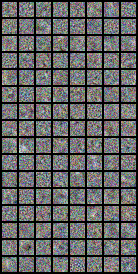
\includegraphics[width=.16\linewidth]{images/convs/beehive.png}
		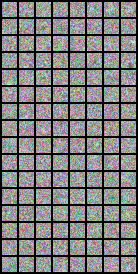
\includegraphics[width=.16\linewidth]{images/convs/rose.png}
		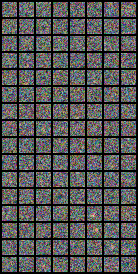
\includegraphics[width=.16\linewidth]{images/convs/coffee.png}
		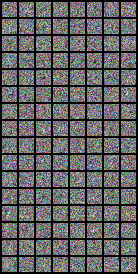
\includegraphics[width=.16\linewidth]{images/convs/bark.png}
        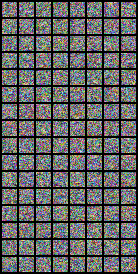
\includegraphics[width=.16\linewidth]{images/convs/water.png}
        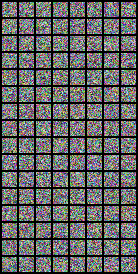
\includegraphics[width=.16\linewidth]{images/convs/stucco.png}
	}\\[3px]
	\caption{Synthesized Images for 1 layer: from epoch 400 to epoch 2000}
\end{figure}

\end{document}
